% Appendix A

\chapter{Appendix}\label{appendixA}
\begin{figure}[!htbp]
\centerline{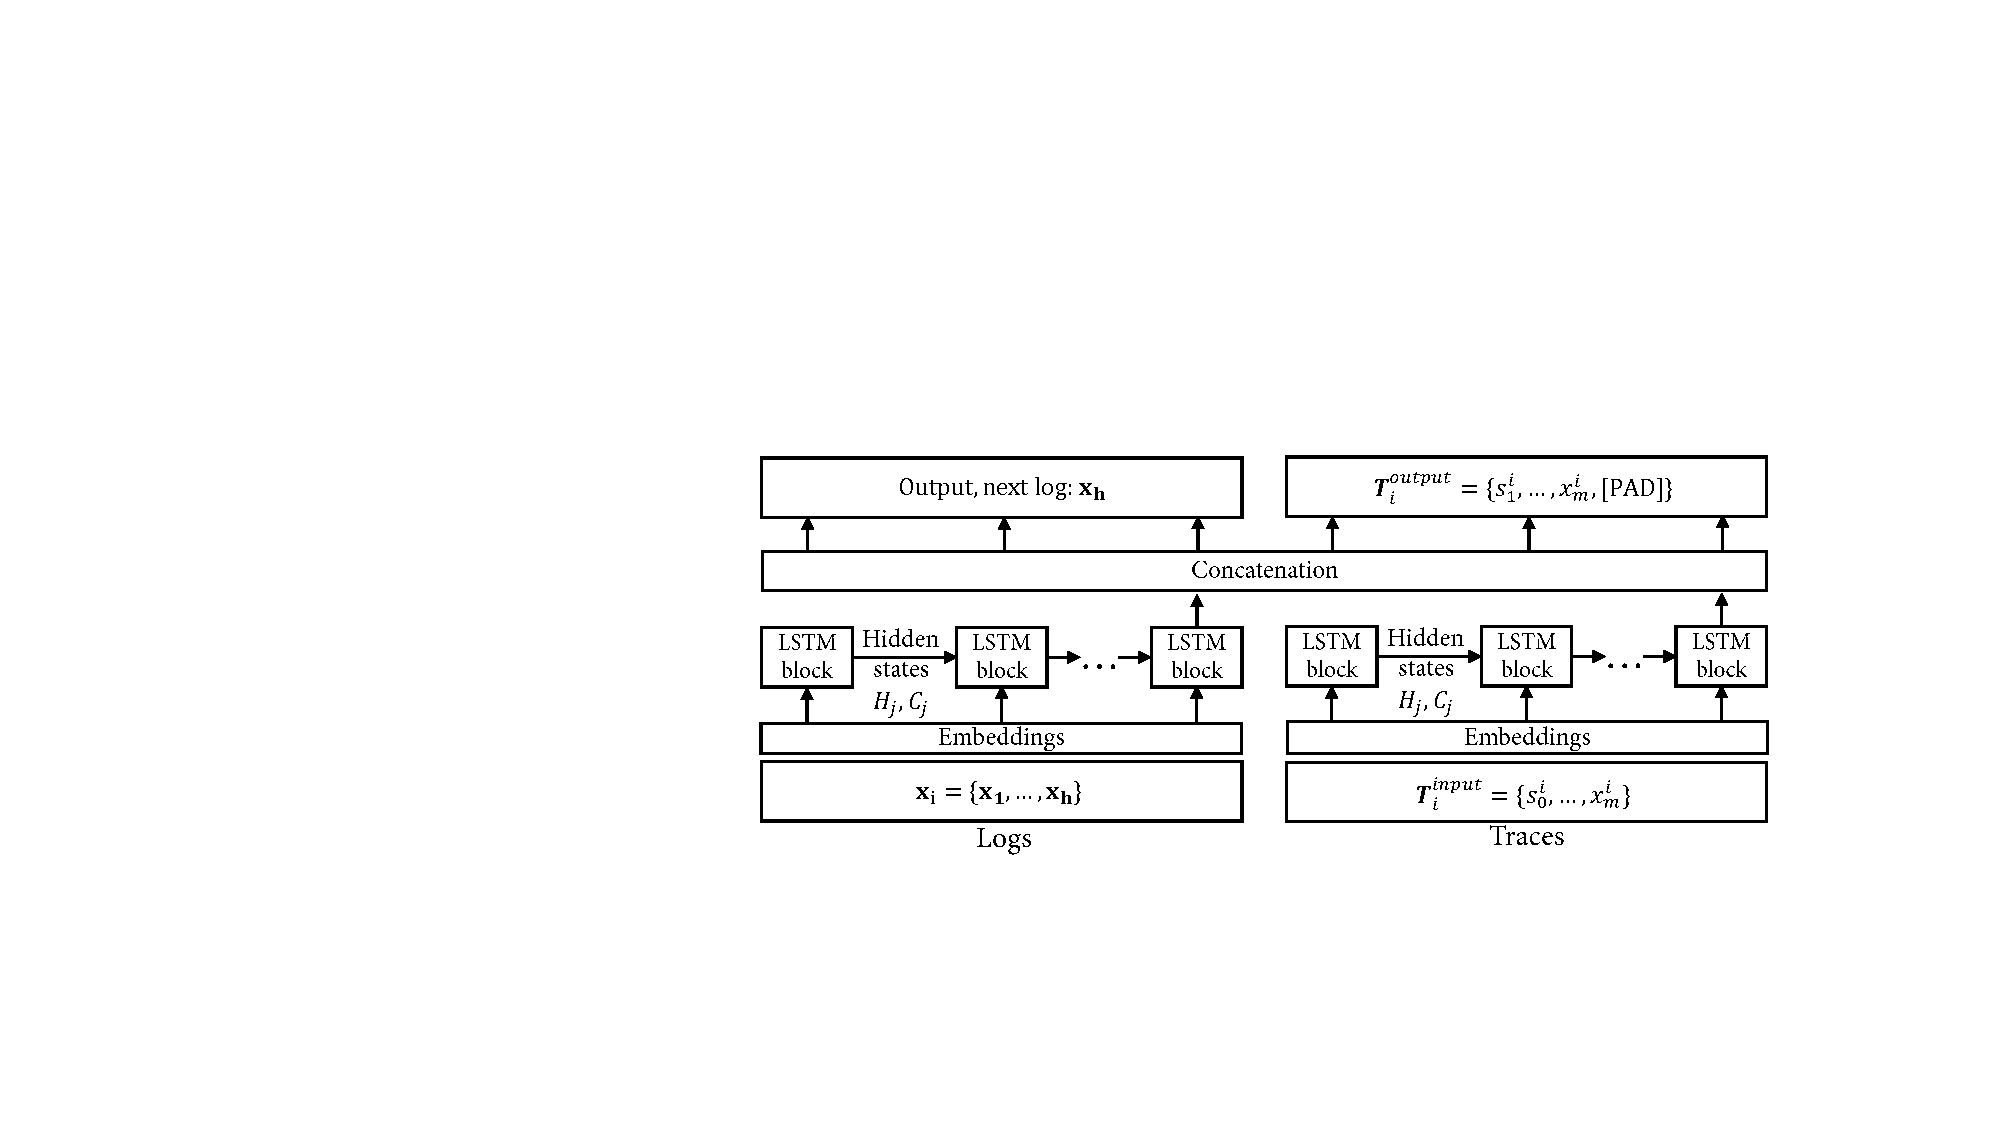
\includegraphics[width=1.0\textwidth]{gfx/chap7/multimodal.pdf}}
\caption{Multimodal LSTM.}
\label{fig:multimodaljoint}
\end{figure}

\section{Multimodal anomaly detection by learning joint representations}
To check if there are possibly abstract correlations that are not captured with rule based logic between the independently trained methods, we designed a multimodal method, described as follows.

We present a multimodal method based on LSTMs~\cite{nedelkoski2020jointmodalities}, which can learn from logs and traces jointly. The purpose of the method is to check whether the learning of joint representations in one model that could possibly utilize the nonlinear correlations between the data types can produce better results than those of  independently trained detectors. 

We depict the method in Figure~\ref{fig:multimodaljoint}.
Sequences of logs and spans are simultaneously provided as inputs to each of the two encoders. The outputs of both encoders are concatenated and fed through an additional linear layer. It uses both representations learned from the encoder to extract joint representations. The shared information from the concatenation is then passed through two linear layers, one for the traces and the other for the logs. The anomaly detection is performed by comparing the predicted output to the observed input, which is used to decide whether an anomaly exists. 

To train the model end-to-end for both modalities, we minimize a cost function that is calculated as an addition of the  cross-entropy losses for the prediction of the next span and log message to appear.

\begin{equation}
    L(joint) = L(logs) + L(traces). 
\end{equation}



\begin{table}[!htbp]
% increase table row spacing, adjust to taste
\renewcommand{\arraystretch}{1.3}
\caption{Results: multimodal LSTM~\cite{nedelkoski2020jointmodalities}.}
\centering
% Some packages, such as MDW tools, offer better commands for making tables
% than the plain LaTeX2e tabular which is used here.
\resizebox{\columnwidth}{!}{%
\begin{tabular}{lcccc}\hline
score  & Logs-multimodal & Trace-multimodal & Single logs & Single traces \\ \hline
accuracy             & 0.976      & 0.990       & 0.974       & 0.955 \\ 
precision            & 0.904      & 0.992       & 0.897       & 0.992 \\ 
recall               & 0.996      & 0.984       & 0.996       & 0.909 \\ 
f1                   & 0.948      & 0.988       & 0.944       & 0.949   \\ \hline
\end{tabular}\label{tab:multimodallstmresults}
}
\end{table}

\section{Results}
Table~\ref{tab:multimodallstmresults} summarizes the results of the experiments. The joint utilization of traces and logs produced comparable results to those of the single-modality anomaly detection methods. The F1-scores of the log data of the multimodal and single methods differed by 0.004, while those for the traces differed by 0.039. The multi-modal LSTM exhibited negligible differences, compared to the independent use of the methods. Therefore, we only evaluated the integration of independently trained detectors and compare to single data source methods. 